\documentclass[11pt]{report}

\usepackage[margin=0.45in]{geometry}

\usepackage{graphicx} % Add pictures to your document
\usepackage{listings}
\usepackage{float}
\usepackage{xcolor}
\usepackage{pgfplots}
\usepackage{sectsty}
\usepackage{hyperref}
\hypersetup{
  colorlinks=true,
  linkcolor=blue,
  filecolor=magenta,      
  urlcolor=cyan,
}

\newcommand{\tux}[1]{\textbf{Tux#1}}

\begin{document}

\title{\huge{\textbf{RCOM Lab2}} \\ Turma 3 // Grupo 3 \\ RCOM 2020/2021 \\ MIEIC FEUP}
\author{João de Jesus Costa \\ \texttt{up201806560} \and
	João Lucas Silva Martins \\ \texttt{up201806436}}
\date{\today{}}

\begin{figure}[b]
  \begin{center}
    
\includegraphics[width=0.6\textwidth]{feup_logo.png}
  \end{center}
\end{figure}
\maketitle{}

\tableofcontents{}
\newpage

{\let\clearpage\relax\chapter{Summary}}

This report documents the project that was developed for the curricular unit
of RCOM (FEUP). We implemented a simple FTP download application and configured
a computer network with three computers, a commercial router and switch.

{\let\clearpage\relax\chapter{Introduction}}

In the first part of this report, we'll focus on the FTP download application
and its architecture.\\
In the second part of this report, we'll focus on the network configuration
and analyze it.

{\let\clearpage\relax\chapter{Part 1 - Download application}}

\section{Architecture}

The application works linearly. We start by opening a socket to the given
server (on the standard FTP port: 21) and authenticate the user. This is
the \textbf{control socket}.\\
After the authentication process, we enter passive mode (with the PASV
command) and open a second socket to the server on the port replied on
the PASV command. This is the \textbf{data socket}.

Once we have this two sockets open, we just need to request the file
we want to the control socket and read it from the data socket. If any
of the steps described fails, the execution is aborted and the user is
informed of the error.

\section{Download steps}
\begin{enumerate}
\item Parse the url and authentication information
\item Resolve the hostname
\item Open control socket to server
\item Authenticate
\item Enter passive mode
\item Open data socket to server
\item Request file on control socket
\item Read file from the data socket
\end{enumerate}

\section{Report of a successful download}

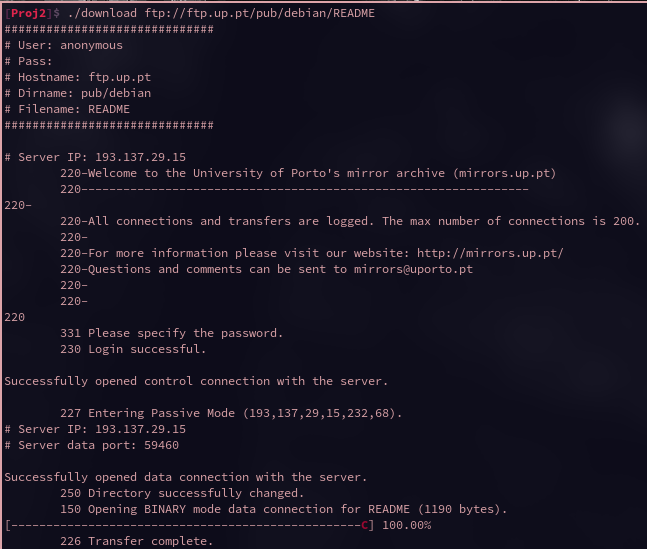
\includegraphics[width=0.65\textwidth]{images/download_report.png}

{\let\clearpage\relax\chapter{Part 2 - Network configuration and analysis}}

This image depicts the cable configuration of the network:

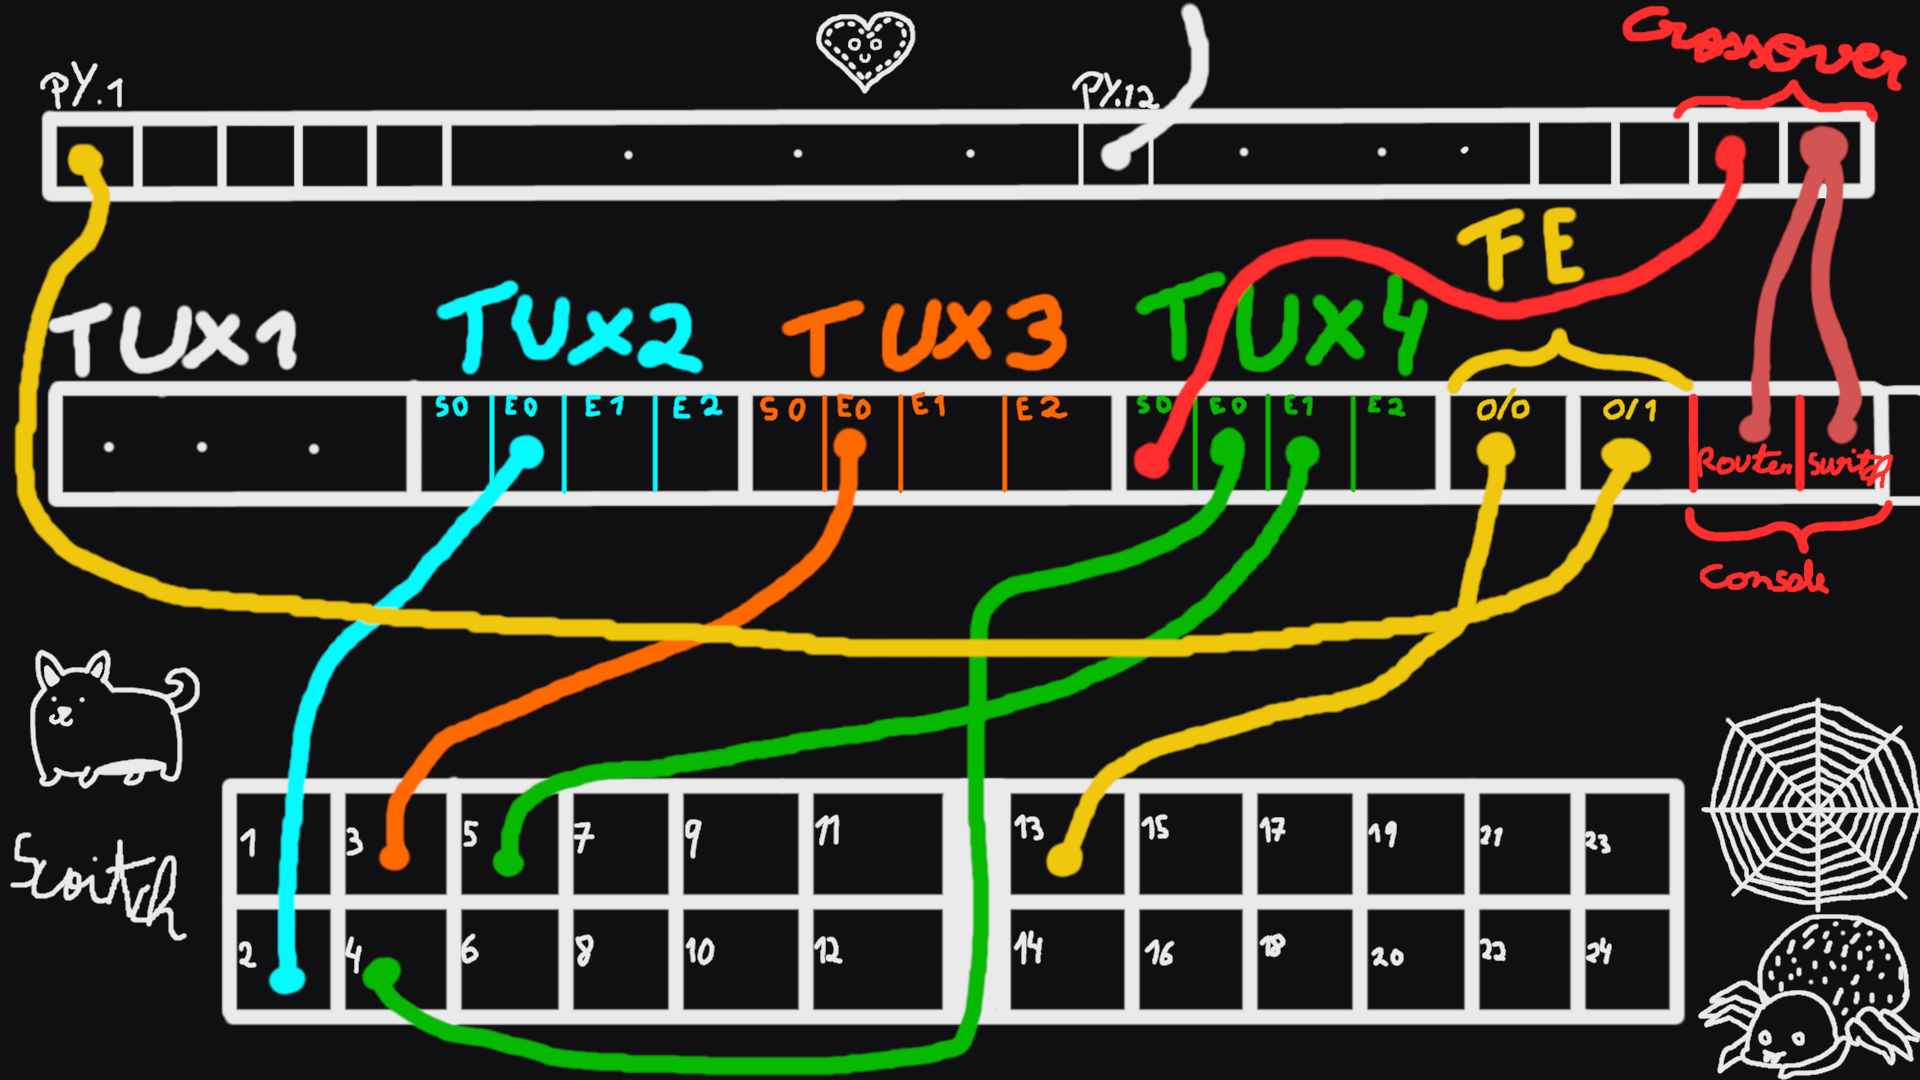
\includegraphics[width=1\textwidth]{images/rcom_proj2_cables.png}

\section{Experience 1 - Configure an IP Network}

\subsection{Objectives}
Connect two hosts to a local network (switch) and enable communication between
them.

\subsection{Configuration commands}
\begin{lstlisting}
# on tux3
ifconfig eth0 172.16.60.1/24

# on tux4
ifconfig eth0 172.16.60.254/24
\end{lstlisting}

\subsection{Questions}
\paragraph{What are the ARP packets and what are they used for?}
ARP packets contain an IP address and are broadcast in the local network
(except to the source host). The host whose IP address is listed in the packet
sends a packet to the source host containing its MAC address. This way,
a host can find the MAC address of a host they only know the IP address of.

\paragraph{What are the MAC and IP addresses of ARP packets and why?}
ARP request packets contain the IP and MAC address of the sender host and the IP
address of the destination host. ARP reply packets include the destination
host's MAC address and are sent back to the source machine.\\
For example, \tux{3} sent an ARP packet asking who has the IP address
$172.16.60.254$. The reply was sent by \tux{4} who had that IP address.

\paragraph{What packets does the ping command generate?}
The ping command generates ICMP ECHO\_REQUEST packet and expect
ICMP ECHO\_RESPONSE packet from a host or gateway.

\paragraph{What are the MAC and IP addresses of the ping packets?}
On the request ping packets, the IP and MAC addresses of the source correspond
to the source host's and the IP and MAC addresses of the destination correspond
to the destination host's. These switch places in the reply packet.\\
For example, \tux{3} sent a ping to the IP address $172.16.60.254$
which corresponds to \tux{4}. The source IP and MAC addresses are
$172.16.60.1$ and $00:21:5a:61:2d:df$ respectively and the destination
IP and MAC addresses are $172.16.60.254$ and $00:21:5a:5a:79:97$
on the request packet.

\paragraph{How to determine if a receiving Ethernet frame is ARP, IP, ICMP?}
We check the EtherType field on the Ethernet header of the MAC frame. The value is
\textbf{0x0800} for IPv4, \textbf{0x0806} for ARP and \textbf{0x86DD} for IPv6.\\
To check if the Ethernet frame contains an ICMP packet, we need to check the
protocol field of the IP packet header. The value is \textbf{1} for ICMP.

\paragraph{How to determine the length of a receiving frame?}
The EtherType field of the header of a Ethernet frame is two octets long and can
have two purposes. Values of less than or equal to 1500 indicate the size of the
payload in bytes. Values above 1536 indicate which protocol is encapsulated in
the payload of the frame. In this second case, the length of the frame can be
determined by determining the length of the encapsulated packet.

\paragraph{What is the loopback interface and why is it important?}
The loopback network specified by the IP protocol has the (IPv4) address
$127.0.0.0/8$. On most IP implementations, any traffic sent to this network
is routed to the same computer. The most commonly used IP address for the
loopback interface is $127.0.0.1$ for IPv4 and $::1$ for IPv6.\\
This interface is useful to test and/or run client-server application/services
on the local machine.

\section{Experience 2 - Implement two virtual LANs in a switch}

\subsection{Objectives}
Connect two hosts to a local network (switch) and enable communication between
them.

\subsection{Configuration commands}
\begin{lstlisting}
# on tux2
ifconfig eth0 172.16.61.1/24
\end{lstlisting}

\subsection{Questions}
\paragraph{How to configure vlan y0?}
\begin{lstlisting}
configure terminal
vlan y0
end

configure terminal 
interface fastethernet 0/3
switchport mode access
switchport access vlan y0
end

configure terminal 
interface fastethernet 0/4
switchport mode access
switchport access vlan y0
end
\end{lstlisting}

\paragraph{How many broadcast domains are there? How can you conclude it from the logs?}
There are two broadcast domains, one for each network (vlan):
$172.16.60.255/24$, $172.16.61.255/24$. If we look at the logs
\textit{exp2\_2\_tux2.pacpng}, \textit{exp2\_2\_tux3.pacpng} and \textit{exp2\_2\_tux4.pacpng},
we can see that when \tux{3} pinged the broadcast of vlan y0, only \tux{4}
got the ping packets. This means that \tux{2} is in a different network, which
has its own broadcast domain.

\section{Experience 3 - Configure a router in Linux}

\subsection{Objectives}
Configure a computer running Linux to act as a router for two networks (vlans).

\subsection{Configuration commands}
\begin{lstlisting}
# on tux2
route add -net 172.16.60.0/24 gw 172.16.61.253 dev eth0

# on tux 3
route add -net 172.16.61.0/24 gw 172.16.60.254 dev eth0

# on tux4
ifconfig eth1 172.16.61.253/24
echo 1 > /proc/sys/net/ipv4/ip_forward
echo 0 > /proc/sys/net/ipv4/icmp_echo_ignore_broadcasts
\end{lstlisting}

\subsection{Questions}
\paragraph{What routes are there in the tuxes? What are their meanings?}
On \tux{2} we have 2 routes: the local network route whose gateway is
$0.0.0.0$ and the route to the \textbf{vlan y0} whose gateway is
\textbf{Tux4's eth1} (IP address $172.16.61.253$). This means \tux{2}
is in \textbf{vlan y1} and needs to send its packets to \tux{4}
when it wants to communicate to \textbf{vlan y0}.\\
On \tux{3} we have 2 routes: the local network route whose gateway is
$0.0.0.0$ and the route to the \textbf{vlan y1} whose gateway is
\textbf{Tux4's eth0} (IP address $172.16.60.254$). This means \tux{3}
is in \textbf{vlan y0} and needs to send its packets to \tux{4}
when it wants to communicate to \textbf{vlan y1}.
On \tux{4} we have 2 routes. Each route corresponds to one local network.
We have two because \tux{4} is in two vlans: y0 and y1.

\paragraph{What information does an entry of the forwarding table contain?}
The table contains gateways and host/networks. Packets destined to a certain host,
are routed to the respective gateway. The gateway might not be directly connected
to the destination, but the host is always directly connected to the gateway.\\
The routes chosen to be in this table are the ones with the best metrics (decided
by the routing algorithm used). This optimizes the connections.

\paragraph{What ARP messages, and associated MAC addresses, are observed and why?}
When the ARP tables of the 3 hosts are clean and \tux{3} pings \tux{2}, we see the
following ARP messages:
\begin{itemize}
  \item \tux{3} asks \tux{4} for his MAC address ($00:21:5a:5a:79:97$), because the
    ping to \tux{2} needs to be routed through \tux{4}.
  \item \tux{4} asks \tux{3} for his MAC address ($00:21:5a:61:2d:df$), because the
    reply to the ping needs to be delivered (it's routed by this host).
  \item \tux{4} asks \tux{2} for his MAC address ($00:22:64:19:02:ba$), because the
    ping destination is \tux{2}.
  \item \tux{2} asks \tux{4} for his MAC address ($00:08:54:71:73:da$), because the
    ping needs to have a reply routed by \tux{4} (to \tux{3}).
\end{itemize}

\paragraph{What ICMP packets are observed and why?}
On the same situation described on the previous answer, we can observe the ICMP packet
(ping) from \tux{3} arriving at \tux{2}. These packets can be seen on both interfaces
of \tux{4} because it routes them from one network to the other.

\paragraph{What are the IP and MAC addresses associated to ICMP packets and why?}
During the transmission, the IP addresses are fixed, because they are part of the
network layer. However, the MAC addresses reflect the hops taken by the packet
through the network. For example, when \tux{3} pings \tux{2}, the source MAC address
is the MAC address of \tux{3} and the destination MAC address is the MAC address
of \textbf{Tux4's eth0} on the first hop. On the second hop, the source MAC address
is the address of \textbf{Tux4's eth1} and the destination address is the address of
\tux{2}.

\section{Experience 4 - Configure a Commercial Router and Implement NAT}

\subsection{Objectives}
Add a commercial router to the network and configure it to use NAT.

\subsection{Configuration commands}
\begin{lstlisting}
# on tux2
route add default gw 172.16.61.254

# on tux 3
route add default gw 172.16.60.254

# on tux 4
route add default gw 172.16.61.254
\end{lstlisting}

\subsection{Questions}
\paragraph{How to configure a static route in a commercial router?}
We use the command $ip route Destination Mask Gateway$, e.g.:
$ip route 172.16.61.1 255.255.255.0 172.16.2.69$.

\paragraph{What are the paths followed by the packets in the experiments carried out and why?}
\begin{itemize}
  \item Step 3
  \begin{itemize}
    \item \tux{3} pings \tux{4}:\\
      \tux{3}($172.16.60.1$) $\rightarrow$ \tux{4}($172.16.60.254$)
    \item \tux{3} pings \tux{2}:\\
      \tux{3}($172.16.60.1$) $\rightarrow$ \tux{4}($172.16.60.254$) $\rightarrow$
      \tux{2}($172.16.61.1$)
    \item \tux{3} pings \textbf{RC}:\\
      \tux{3}($172.16.60.1$) $\rightarrow$ \tux{4}($172.16.60.254$) $\rightarrow$
      \textbf{RC}($172.16.61.254$)
    \item \tux{2} pings \tux{3} with redirects enabled and no gateway route to 172.16.60.0/24 via \tux{4}
      (every ping after the first one):\\
      \tux{2}($172.16.61.1$) $\rightarrow$ \tux{4}($172.16.61.253$) $\rightarrow$ \tux{3}($172.16.60.1$)
  \end{itemize}
  \item Step 4
  \begin{itemize}
    \item \tux{2} pings \tux{3} with redirects disabled and no gateway route to 172.16.60.0/24 via \tux{4}:\\
      \tux{2}($172.16.61.1$) $\rightarrow$ \textbf{RC}($172.16.61.254$) $\rightarrow$
      \tux{4}($172.16.61.253$) $\rightarrow$ \tux{3}($172.16.60.1$)
    \item \tux{2} pings \tux{3} with redirects disabled:\\
      \tux{2}($172.16.61.1$) $\rightarrow$ \tux{4}($172.16.61.253$) $\rightarrow$
      \tux{3}($172.16.60.1$)
    \item \tux{2} pings \tux{3} with redirects enabled and no gateway route to 172.16.60.0/24 via \tux{4} (first ping):\\
      \tux{2}($172.16.61.1$) $\rightarrow$ \textbf{RC}($172.16.61.254$) $\rightarrow$
      \tux{4}($172.16.61.253$) $\rightarrow$ \tux{3}($172.16.60.1$)
    \item \tux{2} pings \tux{3} with redirects enabled and no gateway route to 172.16.60.0/24 via \tux{4}
      (every ping after the first one):\\
      \tux{2}($172.16.61.1$) $\rightarrow$ \tux{4}($172.16.61.253$) $\rightarrow$ \tux{3}($172.16.60.1$)
  \end{itemize}
  \item Step 5. \tux{3} pings the router of lab I.320($172.16.2.254$) without NAT: no route
  \item Step 7. \tux{3} pings the router of lab I.320($172.16.2.254$) with NAT:\\
    \tux{3}($172.16.60.1$) $\rightarrow$ \tux{4}($172.16.60.254$) $\rightarrow$
    \textbf{RC}($172.16.61.254$) $\rightarrow$ \textbf{Router do Lab}($172.16.2.254$)
\end{itemize}

\paragraph{How to configure NAT in a commercial router?}
\begin{lstlisting}
# inside
conf t 
interface fastethernet 0/0
ip address 172.16.61.254 255.255.255.0 
no shutdown 
ip nat inside 
exit 

# outside
interface fastethernet 0/1
ip address 172.16.2.69 255.255.255.0 
no shutdown 
ip nat outside 
exit 

# nat
ip nat pool ovrld 172.16.2.69 172.16.2.69 prefix 24 
ip nat inside source list 1 pool ovrld overload 

# allowed private IP addreses (only until IP 7 on both vlans)
access-list 1 permit 172.16.60.0 0.0.0.7 
access-list 1 permit 172.16.61.0 0.0.0.7 

# routes
ip route 0.0.0.0 0.0.0.0 172.16.2.254 
ip route 172.16.60.0 255.255.255.0 172.16.61.253 
\end{lstlisting}

\paragraph{What does NAT do?}
NAT translates the IP addresses of a private network to a public IP address.
Each private IP address and private port pair is mapped to a public IP address
and public port on the device holding the public IP address. In our case this
public IP address is always $172.16.2.69$.\\
This mapping is bidirectional and stored in the NAT mapping table. Each packet
arriving at the router from `outside' is translated according to the table
and sent to the correct network/host.\\
It should be noted that only allowed private IP addresses can be mapped and that
new entries are added to the NAT table as needed.

\section{Experience 5 - DNS}

\subsection{Objectives}
Configure DNS on hosts running Linux so they can resolve domains on the Internet.

\subsection{Questions}
\paragraph{How to configure the DNS service at an host?}
We need to edit the file $/etc/resolv.conf$ and add all the IP addresses of the DNS
servers we want to use.

\paragraph{What packets are exchanged by DNS and what information is transported?}
There are usually two packets in a DNS exchange. The first is the request packet,
marking the start of a DNS exchange. It contains the domain name of the requested
address and the requested record type (among other things). Next, a response packet
is sent. It includes, among other things, the resolved IP address, assembled
by a query of a name server using the previously given domain name.

\section{Experience 6 - TCP connections}

\subsection{Objectives}
Verify connections to the Internet and test the developed FTP download application.

\subsection{Questions}
\paragraph{How many TCP connections are opened by your ftp application?}
The FTP application creates two TCP connections. The first is created when connecting
to the FTP server through port 21 (default FTP port). It is used to send commands
to the server (e.g.: authentication, entering passive mode, requesting files, etc...)
and reading their replies.\\
The second connection is created when we enter passive mode (by sending the \textbf{PASV}
command to the server). The connection is made to the port replied by the server
upon entering passive mode. We read file contents through this connection.

\paragraph{In what connection is transported the FTP control information?}
The FTP control information is transported in the first connection.

\paragraph{What are the phases of a TCP connection?}
A TCP connection has three phases. The first establishes the connection through
a three-way handshake process. The second is responsible for the transmission
of the data. The third and final phase handles the termination of the
TCP connection using a four-way handshake.

\paragraph{How does the ARQ TCP mechanism work? What are the relevant TCP fields?
What relevant information can be observed in the logs?}
The ARQ TCP mechanism uses the sliding window method to transmit more than one
packet while still waiting for the receiver's confirmation. This is achieved
by storing the last ACKED packet and using it to calculate the size of the
current send buffer. If it surpasses the maximum size of the window,
the sender blocks, waiting for an ACK from the receiver. The wait may be
interrupted by a timeout, with variable length, in which case the sender
attempts to re-transmit the last non-ACKED sent packet.\\
The relevant TCP fields are the window size, the source and destination ports,
the acknowledgment number and the sequence number.\\
In the logs we can verify that the connection establishment (three-way
handshake process) are the first packets in both TCP connections. During
the entire data phase the window size used by the FTP server is mostly
small (229 or 510 bytes), due to the small packet length . However,
during the actual data transfer, the window size rises as expected
to values of 32768 bytes. We can also conclude that there were no timeouts.

\paragraph{How does the TCP congestion control mechanism work? What are the
relevant fields? How did the throughput of the data connection evolve along
the time? Is it according the TCP congestion control mechanism?}
The TCP congestion control mechanism is responsible for controlling
the congestion window, used to calculate the maximum size of the sender's buffer
(minimum between \textbf{CongestionWindow} and \textbf{AdvertisedWindow}).
The congestion window decreases when the network congestion increases,
i.e.: a timeout occurs. Otherwise, the congestion window is increased,
due to the fact that the maximum yield of the network congestion hasn't
been achieved.\\
There are multiple algorithms that specify the amount in which the
congestion window is to be increased/decreased, the most notable are:
Increase/Multiplicative Decrease, Slow Start, and Congestion Avoidance.
The throughput of the data connection remained relatively constant
during the data transfer, rounding 1368 Bytes per TCP packet. These
results are in accordance with the TCP congestion control mechanism
as there were no other connections present. As such, the connection
remained stable during the data transfer.

\paragraph{Is the throughput of a TCP data connections disturbed by the
appearance of a second TCP connection? How?}
When a second TCP connection appears, the throughput has to be divided by
the first and second connections. This means that, depending on how much
data is being transfered for each connection, the throughput can be divided
in half.

{\let\clearpage\relax\chapter{Conclusions}}
The download application developed can download files using the FTP protocol,
reports errors, supports authentication and always closes the connection
gracefully.\\
The network configured allowed us to observe and handle many concepts of
computer networks: vlans, routing, NAT and DNS. The tests using the download
application were successful and we were able to download files on the network
configured.

{\let\clearpage\relax\chapter{References}}
\begin{itemize}
  \item \url{https://en.wikipedia.org/wiki/Ethernet_frame}
  \item \url{https://www.juniper.net/documentation/en_US/junos/topics/concept/interface-security-loopback-understanding.html}
  \item \url{https://en.wikipedia.org/wiki/Transmission_Control_Protocol}
  \item \url{https://upaae.com/how-to-add-and-configure-static-routes-on-cisco-router/}
\end{itemize}

\chapter{Annexes}

\end{document}
